\documentclass[12pt,a4paper,titlepage,final]{article}

% cestina a fonty
\usepackage[czech]{babel}
\usepackage[utf8]{inputenc}
\usepackage[T1]{fontenc}
\usepackage{ae,aecompl}
% balicky pro odkazy
\usepackage[bookmarksopen,colorlinks,plainpages=false,urlcolor=blue,unicode]{hyperref}
\usepackage{url}
% obrazky
\usepackage[dvipdf]{graphicx}
% velikost stranky
\usepackage[top=3.5cm, left=2.0cm, text={17cm, 24cm}, ignorefoot]{geometry}

\begin{document}

%%%%%%%%%%%%%%%%%%%%%%%%%%%%%%%%%%%%%%%%%%%%%%%%%%%%%%%%%%%%%%%%%%%%%%%%%%%%%%
% titulní strana

\def\projname{Implementace interpretu imperativního jazyka IFJ11}
\begin{titlepage}

% \vspace*{1cm}
\begin{figure}[!h]
  \centering
  \includegraphics[height=5cm]{img/logo.eps}
\end{figure}

\vfill

\begin{center}
\begin{Large}
Dokumentace k projektu pro předměty IZP a IUS\\
\end{Large}
\bigskip
\begin{Huge}
\projname\\
\end{Huge}
\begin{large}
projekt č. 2
\end{large}
\end{center}

\vfill

\begin{center}
\begin{Large}
\today
\end{Large}
\end{center}

\vfill

\begin{flushleft}
\begin{large}
\begin{tabular}{ll}
Autor: & \author, \url{\email} \\
 & Fakulta Informačních Technologií \\
 & Vysoké Učení Technické v~Brně \\
\end{tabular}
\end{large}
\end{flushleft}
\end{titlepage}


%%%%%%%%%%%%%%%%%%%%%%%%%%%%%%%%%%%%%%%%%%%%%%%%%%%%%%%%%%%%%%%%%%%%%%%%%%%%%%
% obsah
\pagestyle{plain}
\pagenumbering{roman}
\setcounter{page}{1}
\tableofcontents

%%%%%%%%%%%%%%%%%%%%%%%%%%%%%%%%%%%%%%%%%%%%%%%%%%%%%%%%%%%%%%%%%%%%%%%%%%%%%%
% textova zprava
\newpage
\pagestyle{plain}
\pagenumbering{arabic}
\setcounter{page}{1}

%%%%%%%%%%%%%%%%%%%%%%%%%%%%%%%%%%%%%%%%%%%%%%%%%%%%%%%%%%%%%%%%%%%%%%%%%%%%%%
\section{Úvod}
%%%%%%%%%%%%%%%%%%%%%%%%%%%%%%%%%%%%%%%%%%%%%%%%%%%%%%%%%%%%%%%%%%%%%%%%%%%%%%
Interprety jsou rozsáhlé programy, jejichž implementace spočívá především
v~rozčlenění na~men\-ší celky.

V~tomto projektu bylo naším úkolem vytvořit interpret jazyka IFJ11, který je
podmnožinou jazyka Lua.

Projekt je implementován v~jazyce C. Funguje jako konzolová aplikace, která
načte soubor se~zdrojovým kódem v~jazyce IFJ11 a interpretuje jej. Soubor je
předán jako parametr příkazové řádky.

Při řešení projektu jsme využili poznatků z~předmětů IFJ a IAL.

%%%%%%%%%%%%%%%%%%%%%%%%%%%%%%%%%%%%%%%%%%%%%%%%%%%%%%%%%%%%%%%%%%%%%%%%%%%%%%
\section{Lexikální analyzátor}
%%%%%%%%%%%%%%%%%%%%%%%%%%%%%%%%%%%%%%%%%%%%%%%%%%%%%%%%%%%%%%%%%%%%%%%%%%%%%%
Lexikální analyzátor rozděluje vstupní posloupnost znaků na~lexémy, které
jsou v~praxi repre\-zen\-to\-vány pomocí tokenů. Lexikální analyzátor jsme realizovali
jako konečný automat, který je graficky znázorněn níže. Lexikální
analyzátor je umístěn v~souboru \texttt{scanner.c}.
\begin{figure}[!h]
  \centering
  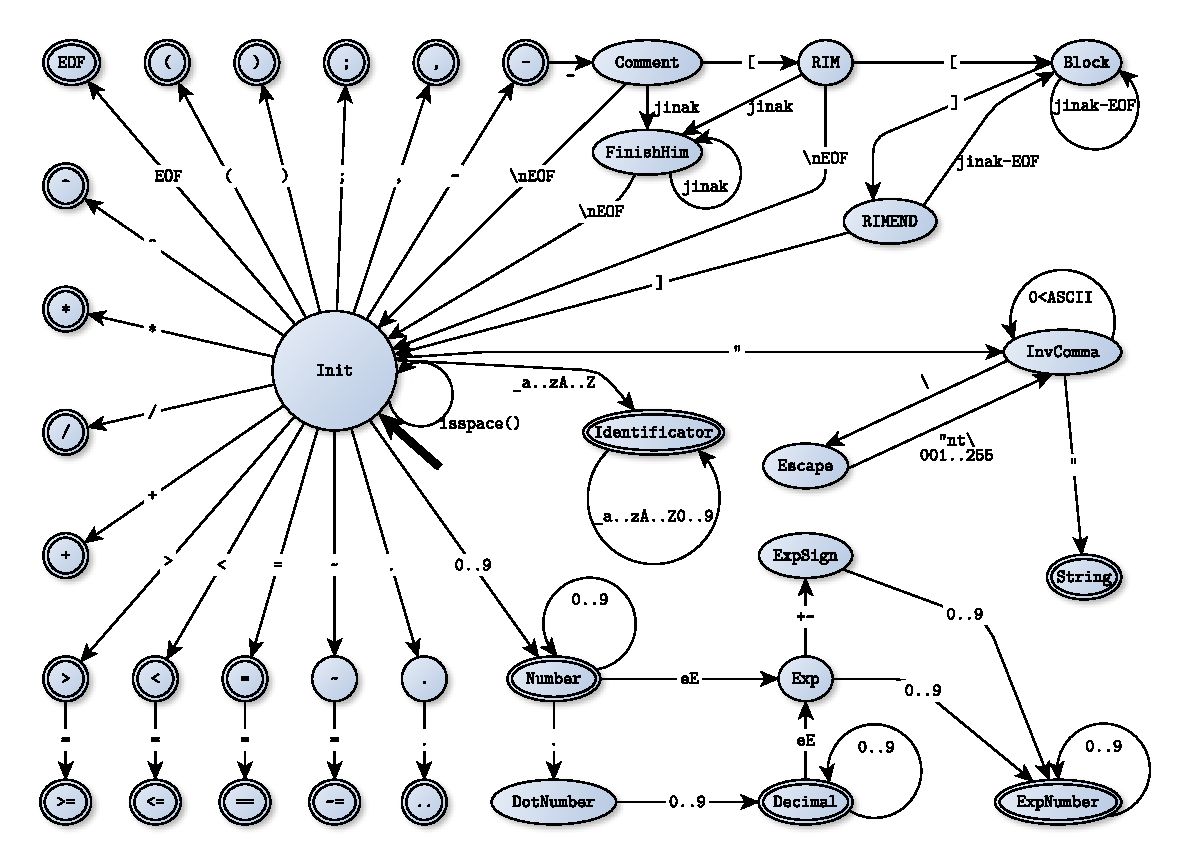
\includegraphics[width=1\textwidth]{img/autom.eps}
\end{figure}

%%%%%%%%%%%%%%%%%%%%%%%%%%%%%%%%%%%%%%%%%%%%%%%%%%%%%%%%%%%%%%%%%%%%%%%%%%%%%%
\section{Syntaktický a sémantický analyzátor}
%%%%%%%%%%%%%%%%%%%%%%%%%%%%%%%%%%%%%%%%%%%%%%%%%%%%%%%%%%%%%%%%%%%%%%%%%%%%%%
Syntaktický analyzátor tvoří z~tokenů datovou strukturu zvanou derivační
strom. Ta je poté využita v~sémantickém analyzátoru, kde je transformována
na~abstraktní syntaktický strom. Zatímco syntaktický analyzátor kontroluje
gramatickou korektnost posloupnosti tokenů, sé\-man\-ti\-cký analyzátor kontroluje
správnost operací.

V~našem interpretu je syntaktická a sémantická analýza rozdělena na~dvě
části. První je umístěna v~souboru \texttt{parser.c} a zpracovává celou strukturu programu
mimo výrazů. Využili jsme metodu rekurzivního sestupu založenou na~LL-gramatice
s~následujícím pravidly.

\begin{flushleft}
\begin{footnotesize}
\begin{tabular}{lll}
\label{synt}
\texttt{<program>}&$\rightarrow$&\texttt{<functlist> "EOF"}\\
\texttt{<functlist>}&$\rightarrow$&\texttt{"function"\ <funct>}\\
\texttt{<funct>}&$\rightarrow$&\texttt{"id"\ "("\ <paramlist>\ <declrlist>\ <functlist>}\\
\texttt{<funct>}&$\rightarrow$&\texttt{"main"\ "("\ ")"\ <declrlist>\ ";"}\\
\texttt{<paramlist>}&$\rightarrow$&\texttt{"id"\ <param>}\\
\texttt{<paramlist>}&$\rightarrow$&\texttt{")"}\\
\texttt{<param>}&$\rightarrow$&\texttt{","\ "id"\ <param>}\\
\texttt{<param>}&$\rightarrow$&\texttt{")"}\\
\texttt{<declrlist>}&$\rightarrow$&\texttt{"local"\ "id"\ <declr>\ <declrlist>}\\
\texttt{<declrlist>}&$\rightarrow$&\texttt{<statlist>\ "end"}\\
\texttt{<declr>}&$\rightarrow$&\texttt{"}\texttt{=}\texttt{"\ <expr>\ ";"}\\
\texttt{<declr>}&$\rightarrow$&\texttt{";"}\\
\texttt{<statlist>}&$\rightarrow$&\texttt{<stat>\ <statlist>}\\
\texttt{<statlist>}&$\rightarrow$&\texttt{"end"}\\
\texttt{<statlist>}&$\rightarrow$&\texttt{"else"}\\
\texttt{<statlist>}&$\rightarrow$&\texttt{"elseif"}\\
\texttt{<statlist>}&$\rightarrow$&\texttt{"until"}\\
\texttt{<stat>}&$\rightarrow$&\texttt{"while"\ <expr>\ "do"\ <statlist>\ "end"\ ";"}\\
\texttt{<stat>}&$\rightarrow$&\texttt{"return"\ <expr>\ ";"}\\
\texttt{<stat>}&$\rightarrow$&\texttt{"write"\ "("\ <exprlist>\ ";"}\\
\texttt{<stat>}&$\rightarrow$&\texttt{"id"\ "}\texttt{=}\texttt{"\ <assign>\ ";"}\\
\texttt{<stat>}&$\rightarrow$&\texttt{"repeat"\ <statlist>\ "until"\ <expr>\ ";"}\\
\texttt{<stat>}&$\rightarrow$&\texttt{"if"\ <expr>\ "then"\ <statlist>\ <ifstat>\ ";"}\\
\texttt{<ifstat>}&$\rightarrow$&\texttt{"end"}\\
\texttt{<ifstat>}&$\rightarrow$&\texttt{"else"\ <statlist>\ "end"}\\
\texttt{<ifstat>}&$\rightarrow$&\texttt{"elseif"\ <expr>\ "then"\ <statlist>\ <ifstat>}\\
\texttt{<exprlist>}&$\rightarrow$&\texttt{<expr>\ <writexpr>}\\
\texttt{<exprlist>}&$\rightarrow$&\texttt{")"}\\
\texttt{<writexpr>}&$\rightarrow$&\texttt{","\ <expr>\ <writexpr>}\\
\texttt{<writexpr>}&$\rightarrow$&\texttt{")"}\\
\texttt{<assign>}&$\rightarrow$&\texttt{"read"\ "("\ "format"\ ")"}\\
\texttt{<assign>}&$\rightarrow$&\texttt{<expr>}\\
\end{tabular}
\end{footnotesize}
\end{flushleft}

V~případě, že se během první části narazí na~výraz \texttt{<expr>}, řízení se předá
druhé části, která zpracovává výrazy. Tato část je zpracována pomocí
precedenční syntaktické analýzy. V~průběhu zpracování výrazu se zpracovává
volání funkce metodou shora dolů dle následujícího pravidla.

\begin{flushleft}
\begin{footnotesize}
\begin{tabular}{lll}
\texttt{<functcall>}&$\rightarrow$&\texttt{"(" [<expr> \{,<expr>\}] ")"}
\end{tabular}
\end{footnotesize}
\end{flushleft}

%%%%%%%%%%%%%%%%%%%%%%%%%%%%%%%%%%%%%%%%%%%%%%%%%%%%%%%%%%%%%%%%%%%%%%%%%%%%%%
\section{Interpret}
%%%%%%%%%%%%%%%%%%%%%%%%%%%%%%%%%%%%%%%%%%%%%%%%%%%%%%%%%%%%%%%%%%%%%%%%%%%%%%
Poslední částí našeho programu je interpret. Během syntaktické a sémantické
analýzy se do~listu instrukcí, který je implementován jako jednosměrný
lineární seznam, přidávají instrukce. Pokud proběhne syntaktická a sémantická
analýza bez chyby, interpret načte jednu instrukci ze~seznamu, vykoná ji a
poté pokračuje na~další instrukci v~seznamu.

%-----------------------------------------------------------------------------
\subsection{Volání funkcí} \label{fcall}
%-----------------------------------------------------------------------------
Volání a návrat z~funkce je ralizován pomocí tří instrukcí. Instrukce \texttt{IMARK}
označí vrchol zásobníku, od~tohoto místa se poté počítají pozice parametrů a lokálních
proměnných. Poté jsou na~zásobník přidány argumenty funkce. Následně se vykoná
instrukce \texttt{ICALL}, která uloží návratovou adresu na~označené místo a
provede volání funkce. Pro~návrat z~funkce poté slouží instrukce \texttt{IRET},
která smaže zásobník až po~označené místo a vloží návratovou hodnotu na~zásobník.

%-----------------------------------------------------------------------------
\subsection{Lokální proměnné a parametry funkcí}
%-----------------------------------------------------------------------------
Hodnoty proměnných a parametrů jsou uloženy na~zásobníku od~posledně označeného
místa instrukcí \texttt{IMARK} v~relativním pořadí jejich deklarací ve~zdrojovém souboru. Pokud má funkce
\texttt{n} parametrů a \texttt{m} lokálních proměnných, pak parametry jsou uloženy na~pozicích
\texttt{1..n} a proměnné na~pozicích \texttt{n+1..n+m}.

K~vložení hodnoty na~zásobník (i literálů) slouží instrukce \texttt{IPUSH}.
Pro~uložení hodnoty z~vrcholu zásobníku do~proměnné slouží instrukce \texttt{IPOP}.

%-----------------------------------------------------------------------------
\subsection{Vyčíslovaní výrazů}
%-----------------------------------------------------------------------------
Pro~vyčíslování výrazů jsme vytvořili 12 instrukcí, kde každá instukce
odpovídá jednomu aritmetickému nebo relačnímu operátoru. Operandy se
berou z~vrcholu zásobníku, kam se následně uloží výsledek operace.

%-----------------------------------------------------------------------------
\subsection{Další instrukce}
%-----------------------------------------------------------------------------
Kromě výše uvedených instrukcí jsme vytvořili 6 instrukcí pro~vestavěné funkce
a příkazy read a write, 2 skokové instrukce pro~nepodmíněný a podmíněný skok
a instrukci \texttt{IHALT} pro~ukončení interpretace.


%%%%%%%%%%%%%%%%%%%%%%%%%%%%%%%%%%%%%%%%%%%%%%%%%%%%%%%%%%%%%%%%%%%%%%%%%%%%%%
\section{Algoritmy do předmětu IAL}
%%%%%%%%%%%%%%%%%%%%%%%%%%%%%%%%%%%%%%%%%%%%%%%%%%%%%%%%%%%%%%%%%%%%%%%%%%%%%%

\subsection{Boyer-Mooreův algoritmus}
Boyer-Mooreův algoritmus je implementován v~souboru \texttt{ial.c} ve~funkci
\texttt{find} a \texttt{computeJumps}. Jedná se o~metodu vyhledání podřetězce v~řetězci.
Pole \texttt{charJump} má velikost 256, což je počet znaků v~ASCII tabulce, a pro~každý
znak obsahuje velikost posunu podřetězce. Funkce \texttt{computeJumps} je pomocná funkce,
která naplní pole \texttt{charJump} podle vyhledávaného podřetězce. Funkce \texttt{find}
porovnává podřetězec zprava znak po~znaku. V~případě neúspěšného porovnání se použije
hodnota posunu z~pole charJump, podřetězec se posune a porovnávání pokračuje.

\subsection{Heap sort}
Řazení metodou Heap sort je implementováno v~souboru \texttt{ial.c} ve~funkcích
\texttt{heapSort} a \texttt{heap\-Extend}. Funkce heapExtend je pomocná funkce, která dokáže
prodloužit haldu o~jeden prvek. Funkce \texttt{heapSort} obsahuje dva kroky. V~obou
krocích je využitá právě pomocná funkce \texttt{heapExtend}. V~prvním kroku je halda
rozšířena na~celé pole. Druhá polovina pole pravidla haldy automaticky splňuje,
několikanásobným voláním funkce \texttt{heapExtend} postupně haldu rozšiřujeme
vždy o~jeden prvek. Ve~druhé fázi vybereme z~haldy největší prvek (ten první)
a vyměníme ho s~posledním prvkem. V~této chvíli jsme však porušili pravidla
haldy a proto musíme znovu zavolat pomocnou funkci \texttt{heapExtend}.

\subsection{Tabulka symbolů implementovaná pomocí hashovací tabulky}
Tabulka symbolů je implementována v~souboru \texttt{ial.c}. Do~tabulky symbolů ukládáme tři
typy symbolů. Symbol typu funkce, typu proměnná a typu literál (konstanta). Pro~každý
typ si uchováváme specifická data. Pro~funkci si ukládáme její adresu a počet
parametrů. Pro~proměnné si ukládáme název funkce ve~které je daná proměnná
deklarovaná a pozici proměnné ve~funkci (jako kolikatý parametr proměnná ve~funkci
vystupuje). Pro~literál si ukládáme jeho typ (string, number, boolean, nil) a jeho hodnotu.

Hashovací funkci jsme převzali z~předmětu IJC, kde byla součástí jednoho z~projektů.
Seznam synonym je zřetězen explicitně do~jednosměrně vázaného lineárního seznamu, kde
se každý nový prvek vkládá na~začátek seznamu. Velikost hashovací tabulky je zvolena
jako prvočíslo 193, což by měla být adekvátní velikost pro~běžné programy.

%%%%%%%%%%%%%%%%%%%%%%%%%%%%%%%%%%%%%%%%%%%%%%%%%%%%%%%%%%%%%%%%%%%%%%%%%%%%%%
\section{Rozšíření}
%%%%%%%%%%%%%%%%%%%%%%%%%%%%%%%%%%%%%%%%%%%%%%%%%%%%%%%%%%%%%%%%%%%%%%%%%%%%%%
V rámci projektu jsme se rozhodli implementovat následující rozšíření:
\begin{itemize}
  \item IFTHEN
  \item FUNEXP
  \item LOCALEXPR
  \item REPEAT
\end{itemize}

Rozšíření jsou vyřešena dodatečnými pravidly v LL-gramatice, viz sekce \ref{synt}.
Těmi je vyřešen i problém návaznosti příkazu \texttt{else} a \texttt{elseif}, který se přiřadí
k poslednímu příkazu \texttt{if} případně \texttt{elseif}.

Pro~tato rozšíření jsme se rozhodli ještě před~implementací parseru a zabudovali jsme je rovnou
při~jeho implementaci.

Při~rozšíření \texttt{FUNEXP} jsme se museli zamyslet nad~voláním funkcí, viz sekce \ref{fcall},
a také nad~zpracováním volání funkce ve~výrazu. To je implementováno v~souboru \texttt{expr.c}
ve~funkci \texttt{functcall}, která se zavolá ve~chvíli, kdy se při~zpracování výrazů narazí
na~identifikátor funkce. Tato funkce kontroluje syntaxi volání a počet zadaných argumentů, po~překročení
počtu parametrů volané funkce již pro~další argumenty negeneruje instrukce. V~případě
nedostatku argumentů, doplní chybějící počet konstantou \texttt{NIL}.


%%%%%%%%%%%%%%%%%%%%%%%%%%%%%%%%%%%%%%%%%%%%%%%%%%%%%%%%%%%%%%%%%%%%%%%%%%%%%%
\section{Práce v týmu}
%%%%%%%%%%%%%%%%%%%%%%%%%%%%%%%%%%%%%%%%%%%%%%%%%%%%%%%%%%%%%%%%%%%%%%%%%%%%%%
Náš tým se dal dohromady velmi prozaickým způsobem. Chodili jsme na~stejné gymnázium,
 sedávali jsme spolu na~přednáškách, a tak při skládání týmu nebylo co řešit.

První problém, se kterým jsme se v~týmu potkali, byla role vedoucího.
Nikdo se totiž na~tuto pozici nijak netlačil, což vyvrcholilo tím, že jsme se
při~přihlašování vedoucích přihlásili rovnou dva (prostě proto, aby tam aspoň někdo byl).
Naštěstí se dalo po~uzávěrce ještě odhlásit, takže jsme se nakonec i oficiálně šťastně
potkali v~jednom týmu.

Rozdělení práce probíhalo hlavně na~bázi \uv{když se někomu chce, tak ať něco udělá}.
První oficální rozdělení proběhlo někdy v~půlce října, kdy jsme se rozdělili na~dvě
dvojice, z~nichž jedna dělala interpret a druhá lexikální analyzátor.

Domluva v~týmu probíhala hlavně na~pondělních přednáškách a ve~středu ve~dvouhodinové
pauze mezi dvěma přednáškami. Ke~komunikaci jsme už někdy v~září vytvořili i diskuzní
fórum, které zůstalo na~celém jednom příspěvku. Mimo osobní domluvu jsme komunikovali
ještě \mbox{e-mailem}.

K~uchovávání aktuálního stavu projektu jsme používali svn na~školním serveru merlin.
Měli jsme snahu zaznamenávat až větší změny, abychom měli méně commitů, přesto se jejich
počet vyšplhal na~49.

%%%%%%%%%%%%%%%%%%%%%%%%%%%%%%%%%%%%%%%%%%%%%%%%%%%%%%%%%%%%%%%%%%%%%%%%%%%%%%
\section{Závěr}
%%%%%%%%%%%%%%%%%%%%%%%%%%%%%%%%%%%%%%%%%%%%%%%%%%%%%%%%%%%%%%%%%%%%%%%%%%%%%%

Tento projekt pro~nás byl jednoznačně pozitivní zkušeností. Naučili jsme se spolupracovat
ve~skupině lidí a vytvářet společně větší projekty obsahující více navzájem kooperujících modulů.

Program byl testován na~několika zdrojových kódech jazyka IFJ11 a všechny proběhly v~pořádku.
Doufáme, že tomu tak bude i u~těch, které budou použity při~testování správnosti programu.
%%%%%%%%%%%%%%%%%%%%%%%%%%%%%%%%%%%%%%%%%%%%%%%%%%%%%%%%%%%%%%%%%%%%%%%%%%%%%%
% přílohy
\appendix

\section{Metriky kódu} \label{metriky}
\paragraph{Počet souborů:} 24 souborů
\paragraph{Počet řádků zdrojového textu:} 4423 řádků
\paragraph{Velikost statických dat:} 31444B
\paragraph{Velikost spustitelného souboru:} 39612B (systém Linux, 64 bitová
architektura, při pře\-kla\-du bez~ladicích informací)


\end{document}
